\section{Selvlærende modeller}
% Introduktion til andre mulige modeller
Der findes alternative modeller som kan blive implementeret i et system, der er værd at undersøge. Disse udvalgte alternative modeller er maskinlæring og evolutions algoritmer. I dette afsnit vil disse to modeller blive belyst, hvor der til slut vil blive argumenteret og vurderet for hvilken model som projektet gør brug af.
 
\subsection{Maskinlæring}
% Introduktion og definition
% Maskinlæring er et meget bredt område, derfor gennemgår vi nogle forskellige dele af emnet
Modellen for maskinlæring består af at systemet lærer fra udføre opgaver og hvor effektivt systemet kan dette. Denne proces kan udtrykkes i følgende definition:

\say{\textbf{Definition}: A computer program is said to \textbf{learn} from experience \textit{E} with respect to some class of tasks \textit{T} and performance measure \textit{P}, if its performance at tasks \textit{T}, as measured by \textit{P}, improves with experience \textit{E}} \citep{Mitchell1997}

% Hvad er maskinlæring og hvor kommer det fra
Maskinlæringsalgoritmer stammer tilbage fra 1950'erne, hvor IBM-forskeren, Arthur Lee Samuels, opfandt den tidligste maskine, som kunne spille et damspil ved hjælp af maskinlæringsalgoritmer. Siden dengang er kunstig intelligens blevet drastisk udviklet og har et stort potentiale i dag, grundet mange årsager. En af disse årsager er, at man i dag har store mængder data, som er gjort tilgængelige til kommerciel brug og nu kan bevares billigt. Samtidig er moderne processorer meget mere kraftfulde og kan analysere data på rekordtid. På grund af, at maskinlæring er blevet så omtalt, er der nu mange open-source brugervenlige bibliotekter som er gjort tilgængelige \cite{ML1}.
\par
Maskinlæring bruges eksempelvis inden for e-handel, når maskinen lærer at promovere produkter på en hjemmeside. En model kunne være, at et system skal promovere produkter ud fra anmeldelser, kundens søgehistorik og måske anbefale produkter ud fra, hvad andre har købt sammen med et given produkt \cite{ML1}.
\par
Et andet område, som maskinlæring dagligt bruges indenfor, er eksempelvis Youtube, som er ejet af Google. En artikel udgivet af Google omhandler, hvordan maskinlæring anvendes til at anbefale seere nye videoer, baseret på deres adfærd. Google beskriver deres system som værende et af de største og mest sofistikerede systemer der eksisterer \cite{ML2}.
\par
Der findes også forskellige moddeller for hvor maskinlæring anvendes. Disse modeller betegnes ved supervised-, unsupervised-, reinforcement- og neural network learning.

\subsubsection{Supervised learning}
\textit{Supervised learning} er en træningsmetode der bliver givet et datasæt, hvori de rigtige resultater er markerede, så træningsalgoritmen ved, hvordan den skal tilrette modellen der trænes. Dette kan sammenlignes med et menneske, som lærer ved at få feedback fra en underviser, som kender de rigtige svar \citep{Jeanmonod2018}. Et ofte brugt eksempel på et sæt af træningsdata er Iris-datasættet fra \cite{fisher1936}. Ved at bruge dette datasæt til at træne en læringsalgoritme, vil det blive i stand til at klassificere, hvilken af de tre arter i datasættet, som en irisblomst tilhører, ud fra mål af kron- og bægerblade.
\par
% Afgrænsning - foretages også længere nede, så er måske ikke nødvendig her.
Supervised learning fravælges som metode i dette projekt, da der ikke er let tilgængelige datasæt med markeret data, der omhandler adfærd af sværme. Desuden er det uden for projektets rammer at sammensætte et tilstrækkeligt datasæt til dette formål. 

\subsubsection{Unsupervised learning}
% Lidt mere intro til unsupervised her.
\textit{Unsupervised learning} får, ligesom supervised learning, data som computeren kan arbejde med. Forskellen på disse to er, at unsupervised learning ikke får nogen mærkater på de data, der skal trænes på. Altså kan den ikke på samme måde trænes op, da den ikke kender resultaterne på eventuelle træningsdata. Der skal her laves analyser på data, og det kan derefter sorteres i undergrupper, hvilket kunne gøres ved hjælp at et beslutningstræ (eng. decision tree). Et beslutningstræ er et godt eksempel på, hvordan unsupervised learning foregår, da programmet her skal finde nogle bestemte mønstre, som den skal gennemgå for alle data. 

% Afgrænsning
Sortering af data i undergrupper, er ikke en tilgang der egner sig til at modellere sværme. Derfor fravælges unsupervised learning som fremgangsmåde i dette projekt.

\subsubsection{Reinforcement learning}
Ved denne type af læring, starter modellen typisk med en ren tavle \cite{deep-reinforcement-learning}. Modellen får ingen data med markerede svar, som i supervised learning, men skal i stedet prøve sig frem. En vigtig del af reinforcement learning, er at modellen får feedback på de handlinger den foretager. Dette sker igennem en fitness-funktion, som belønner modellen alt efter hvor tæt på målet den er. Dette kunne eksempelvis være hvor hurtigt modellen kan finde vej, fra ét punkt til et andet, eller hvor tæt den er på at gætte en tekststreng, eller hvor langt en simuleret bil har kørt [CITATION]. Fitness-funktionen beregner derefter en fitness-værdi, ud fra hvor godt modellen klarede sig, og ud fra denne feedback, kan modellen justere sig selv, og prøve igen, indtil den kommer i mål. Der findes utallige applikationer for denne type maskinlæring, dog skal der være et klart mål med modellen, noget programmøren gerne vil optimere, da modellen skal bruge en fitness-funktion for at kunne fungere \cite{deep-reinforcement-learning}. 

% Policy based
% Value based
% Model based
Der findes tre forskellige tilgange til reinforcement learning benævnt value based, policy based og model based. Værdibaseret (value based) tager udgangpunkt i at optimere en værdifunktion vis funktion udregner den forventede gevinst. Maskinen vil derfor komme frem til de handlinger som giver den største gevinst baseret på funktionen. Hvis der bliver tilføjer en "policy" funktion sammen med værdifunktionen, så er det en policy based reinforcement learning tilgang. Her forsøger maskinen at optimere både sin policyfunktion uden at værdifunktionen går tabt. Policyfunktionen udregner hvilken handling maskinen skal tage ud fra input fra eksempelvis værdifunktionen. Under policyfunktioner findes der to typer heraf benævnt deterministic og stochastic. En deterministic funktion vil altid give den samme baseret på de samme inputs, mens en stochastic funktion har en sandsynlighed involveret. Denne sandsynlighed resultere i at der kan forekomme flere handlinger ud af den samme funktion. Endeligt findes der en model baseret tilgang hvor der bliver lavet en model af miljøet som beskriver opførelsen for miljøet. \cite{RLapproaches}

% Afgrænsning?
Tilgangen omkring reinforcement learning handler fundamentalt set om at optimere en process på baggrund af en fitness og gevinst. Problemet med denne model er at brugeren ikke kan se årsagen og baggrunden for en bestemt handling som maskinen foretager sig grundet en black box. Denne black box indeholder mange sandsynligheder og udregninger som er svære at fortolke. Derfor afgrænses der væk fra denne tilgang.

\subsubsection{Neural Network Learning} % Det her skal nok kortes ned
En anden tilgang til maskinlæring er kunstige neurale netværk, der kan bruges til både supervised, unsupervised og reinforcement learning. Denne tilgang er inspireret af, hvordan en biologisk hjerne er opbygget. Et kunstigt neuralt netværk består i korte træk af en række lag. Ethvert neuralt netværk vil have mindst to lag, et input lag og et outputlag. Imellem disse to kan der være et antal skjulte lag. Hvert af disse skjulte lag indeholder et antal neuroner \cite{E1997}, der består af en aktiveringsfunktion. Figur \ref{NeuralNet} side \pageref{NeuralNet} illustrerer hvordan et neuralt netværk er bygget op i lag og neuroner.
\par
% Kort forklaring af aktiveringsfunktion
Aktiveringsfunktionen er den funktion der behandler en neurons inputværdier. Resultatet af denne funktion er neuronens output. Antallet af neuroner i det første lag baseres på strukturen og mængden af inputdata, mens antallet i det sidste lag er baseret på hvordan resultatet er repræsenteret.
\par
Neuronerne i et skjult lag modtager information fra én eller flere neuroner i det foregående lag, og giver selv information videre til én eller flere neuroner i det efterfølgende lag. Resultatet af en aktiveringsfunktion i en neuron, bliver først ændret i forhold til en vægt og et eventuelt bias. Denne vægt og bias er forskellig for hver forbindelse mellem to neuroner. Det er disse vægte og bias, som ændres under træningsprocessen, der eksempelvis foregår ved en metode ved navn \textit{backpropagation}.
%%%%%%
\begin{figure}[H]
    \centering
    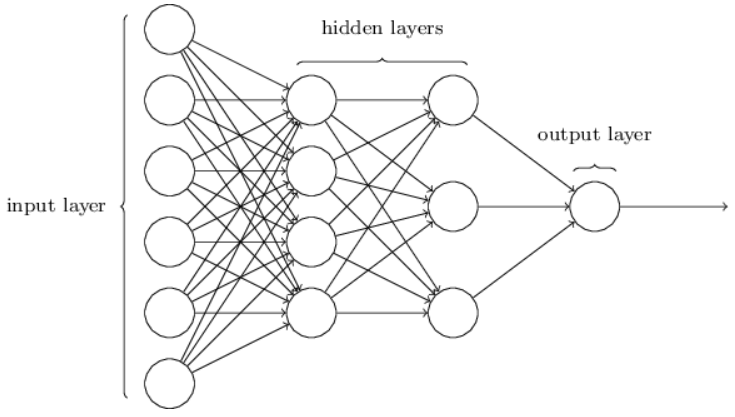
\includegraphics[width=0.7\textwidth]{figures/NeuralNetIMG.PNG}
    \caption{Billedet er fra \cite{Nielsen2015}, og viser et eksempel på opbygningen af et neuralt netværk med to skjulte lag.}
    \label{NeuralNet}
\end{figure}
%%%%%%
% Kort forklaring af backpropagation 
Backpropagation er en metode der bruges til at udregne gradienten i et feed-forward neuralt netværk \cite{Nielsen2015}. Denne gradient beskriver hvordan vægtene og bias i det neurale netværk skal justeres, for at resultatet bevæger sig mod en optimal løsning. 
\par % Næste sætning skal specificeres, så det også kan anvendes hvis man ikke kender svarene
Et neuralt netværk trænes med backpropagation ved at afgøre, hvor stor fejlen er i det sidste lag i netværket, eksempelvis ved at sammenligne med markerede resultater, eller en fitness-værdi. Herefter propageres der baglæns i netværket, ved at udregne fejlen i et lag, ud fra fejlen i det efterfølgende lag \cite{Nielsen2015}. Resultatet af denne backpropagation er som sagt en gradient der angiver, hvordan vægte og bias i de enkelte lag skal justeres, for at optimere resultatet. 
\\\\
% Herfra og ned til "Valg af læringsmetode", skal vi måske overveje hvordan det skal gøres
% Her bliver træningsfunktionen givet et datasæt med mærkater. Den ved altså, hvad der hænger sammen med hvad.

% Bedøm om dette afsnit skal med og om det skal udvides.
% Kunstige neurale netværk er i stand til at approksimere en hvilken som helst funktion \cite{LESHNO1993861}.
Ideen omkring kunstige neurale netværk kan bruges indenfor supervised, unsupervised og reinforcement learning \cite{dey2016machine}. 
\par
Supervised Neural Network er konceptet hvor et neuralt netværk bliver brugt indenfor supervised learning. Når netværket trænes, får det data fra et træningseksempel, og netværkets resultat sammenlignes med det markerede resultat for træningseksemplet. Herefter foretages der justeringer i det neurale netværk med backpropagation sådan at optimal næste gang \cite{dey2016machine}.
\par
Unsupervised Neural Network er også en tilgang, hvor det neurale netværk bliver brugt indefor unsupervised learning. Her sammenligner det neurale netværk de forskellige inputs og grupperer dem, ud fra fællestræk \cite{dey2016machine}.
\par
Reinforced Neural Network konceptet er hvor det neurale netværk bruges indenfor reinforcement learning. Her bruges fitness-værdien for et resultat, til at ændre vægtene i det neurale netværk. Hvis fitness-værdien er høj vil det output i det neurale netværk forstærkes\cite{dey2016machine}. 
\par
Et eksempel på hvor maskinlæring og konceptet omkring neurale netværk anvendes, er AlphaStar som består af reinforced og supervised neurale netværk. AlphaStar, som er lavet af Google DeepMind, vandt 5-0 i StarCraft 2 over Grzegorz "MaNa" Kominczover, som er en af verdens bedste spillere. Kunstig intelligens har haft stor succes i Atari spil, Mario og Dota 2, men har haft problemer StarCraft 2, fordi det er et meget komplekst spil. Men nu i januar 2019 har kunstig intelligens også haft stor succes her \cite{AlphaStar}.

\subsection{Evolutionsalgoritmer}\label{subsec:Evolutionsalgoritmer}
% Det skal overvejes hvad der skal være i dette afsnit, og hvad der skal være i det mere dybdegående afsnit.
Evolutionsalgoritmer er en metaheuristik, der er inspireret af biologisk evolution. % Hvad er en metaheuristik?
Der findes flere underkategorier inden for evolutions algoritmer, en illustration af disse kan ses på figur \ref{EA-Kategorier}. Fælles for algoritmerne i de forskellige underkategorier af evolutions algoritmer er, at de har en befolkning af mulige løsninger. De enkelte enheder i befolkningen starter typisk med at være tilfældige, men udvikles over flere generationer, gennem en række processer \cite{DBLP:journals/corr/abs-1805-11014}.
\par
De processer der udføres på en befolkning er reproduktion, mutation, konkurrence og selektion \cite{Back1999}, og de kaldes samlet set for \textit{genetiske operatorer}. De er hvad der gør at evolutions algoritmer minder om biologisk evolution. Forløbet starter som sagt med at danne en initierende befolkning af mulige løsninger tilfældigt. De mulige løsninger bedømmes ved brug af en fitness-funktion, ligesom det er tilfældet med reinforcement learning. Konkurrence og selektion bruges til at udvælge hvilke medlemmer af befolkningen, der skal reproducere og danne den næste generation. Under denne reproduktion er der en chance for mutation, der ændrer på afkommet.
\par
% Lidt om genetik inden for evolutions algoritmer
Et andet koncept der bruges inden for visse underkategorier af evolutions algoritmer, er genetik. Disse underkategorier er bl.a. genetiske algoritmer og genetisk programmering.
Disse algoritmer bruger yderligere biologisk inspirerede processer såsom nedarvning, kromosomer og overkrydsning. Disse processer bruges til at kombinerer arvematerialet fra to forældre, med det formål at danne afkom der er i stand til at løse opgaven bedre. 
\par
% Afsnit der beskriver vektorbaserede tilgange, med evolutions strategier som eksempel
En anden type af evolutions algoritmer er vektorbaserede evolutions algoritmer. Et eksempel på en sådan algoritme, er evolutions strategier. Til forskel på de genetisk baserede tilgange, bruger denne biologiske analogier på makro-niveau. På dette niveau er der tale om operatorer såsom variation og nedarvning, og gør ikke brug af genetiske egenskaber som kromosomer eller gener \cite{Brownlee2011}. De mulige løsninger i en befolkning, bliver repræsenteret af vektorer, og behandles ved at fortage operationer på disse vektorer. 

%%%%% Figur der viser (nogle) underkategorier inden for Evolutions Algoritmer
\begin{figure}[H]
    \centering
    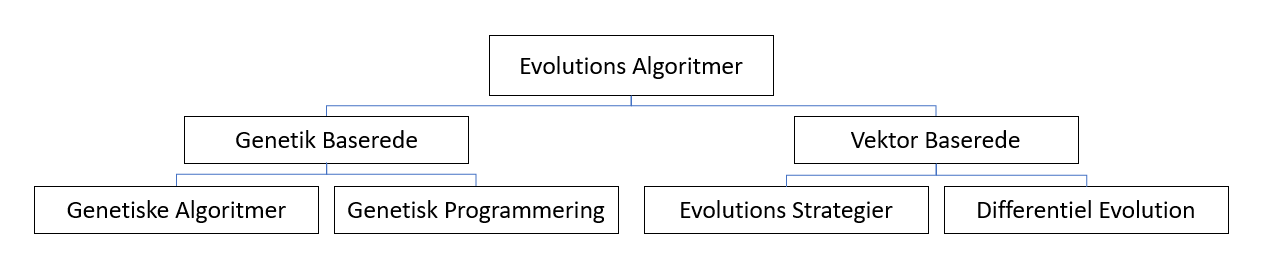
\includegraphics[width=1\textwidth]{figures/EA-kategorier.PNG}
    \caption{Figuren viser viser en illustration af nogle af de underkategorier der er under evolutions algoritmer. Til          venstre er de genetisk baserede, og til højre er de vektor baserede.}
    \label{EA-Kategorier}
\end{figure}
%%%%%

% Bedømmelse af evolutionsalgoritmer
Evolutions algoritmer er en lovende tilgang til at simulere adfærden i sværme, da der er fokus på at optimere hvordan medlemmerne i befolkningen løser problemet. Der stilles krav til at der skal være en fitness-funktion, der kan bruges til at bedømme befolkningen. Desuden er det nødvendigt at definere hvilke egenskaber en befolkning har, da det er disse er ændres under optimeringen. Det er ikke nødvendigt at have kendskab til, hvordan disse egenskaber påvirker opførslen af befolkningens medlemmer. Hvilket betyder at evolutions algoritmer kan bruges til at undersøge hvordan og hvorfor sværmadfærd opstår.

% Herfra og ned, omtaler elementer der specifikt vedrør genetiske algoritmer
% Ud fra denne fitness-værdi, bestemmes det med en udvælgelsesmetode, hvilke løsningsmuligheder, der skal reproducere, og danne nye løsningsmulighder i den næste generation. Produktet af denne reproduktion kan bestemmes på flere forskellige måder. En måde er at tage gennemsnittet af forældrenes arvemateriale og lade dette blive afkommets arvemateriale, en anden måde er at blande forældrenes arvemateriale. Når der skabes en ny befolkning, er der en chance for at afkommet muterer, og dermed introducerer nyt arvemateriale. Chancen for denne mutation er typisk fastlagt som en hyperparameter. Der bliver dannet nye generationer, indtil at resultatet er blevet acceptabelt. 

\subsection*{Andet?}
% Vi kunne beskrive noget som particle swarm optimization, eller ant colony - hvad-end-det-nu-hed, hvis det er nødvendigt at have mere med.
\todo[inline]{Se her!}

\subsection{Mini-konklusion}
% Skal skrives om, så det opsamler på de muligheder vi har skitseret i afsnitet forinden, og sige hvorfor vi gør som vi gør
\todo[inline]{Hallo her!}
På baggrund af gennemgangen ovenfor, kan der nu foretages en afgrænsning til en bestemt tilgang inden for maskinlæring. % Automatisk læring
\par
Supervised learning kan siges at være en mindre relevant metode for vores projekt af lignende årsager til fravalget af den regelbaserede tilgang (reference til afsnittet ovenfor): Kravet om præmarkeret data, feature selection eller lign. er vanskeligt at imødekomme uden at have konkret kendskab til grundlaget for dynamikken i den pågældende sværm. Problemløsningen risikerer altså at blive cirkulær, og vi vælger derfor superviseret maskinlæring fra. % Den ville blive cirkulær hvis man man brugte svaret til at finde svaret. Men er grunden til at vi valgte det fra ikke at vi ikke har noget data, og derfor slet ikke kan starte?
\par
Unsupervised learning kræver ikke, at der arbejdes med prædefinerede kategorier. Kategorier i form af klynger, associationsdannelser eller lignende er som sagt typisk enderesultatet. Imidlertid synes abstrakt kategoridannelse ikke at være den mest nærliggende måde at rammesætte kerneproblemet om at simulere de lokale interaktioner i sværme. Problemet med at modellere på denne måde forstærkes af, at sværme ofte består af dyrearter hvis adfærd ikke er baseret på abstrakt tænkning: Fisk, insekter, fugle og lignende (se Indledningen). % Forkortelser
Tilgangen fravælges altså, fordi simulationen af de levende agenter nemt risikerer at få lav \textit{økologisk validitet}. Dvs. en vis kunstighed, der giver lav udsagnskraft om det naturfænomen, der simuleres \cite{brewer2014}.
\par
Reinforcement learning synes derimod at være en relevant tilgang, der er værd at undersøge nærmere. Tilgangen har et iboende fokus på at optimere agenters evne til at respondere på et omskifteligt miljø. Der lægges altså mere op til simulering af levende agenter end ved Unsupervised learning. Ydermere defineres tilgangen ikke af forudbestemte kategorier, mærkater og tilsvarende ligesom ved Supervised learning. 
\par
Derfor foretrækkes reinforcement learning fremfor alt andet af ovenstående grunde. Projektet vil fremover arbejde videre med denne tilgang. % Vi vælger ikke reinforcement learning, pga. black box problemet

% Evolutionsalgoritmer afgrænsning
